\chapter{Figures}
\label{cha:app_figures}

This appendix contains several figures that were not considered relevant enough to be part of the main text.

\section{Figures of disconnected meanings for the \secondmodel{}}
\label{sec:app_figures_second-model}

Section \ref{sec:results_new_other} shows the results obtained for the current model.
For comparison with \cite{Ferrer2003a}, figures generated from the same sets of parameters as for the \secondmodel{}  but with disconnected meanings kept disallowed are shown here.
The single connection initial state is never shown, as it is an invalid configuration.

For the case $\phi=0$, Figures \ref{fig:informationTheoretic_uniform_phi0_nm400_dynamic_randomBipartite_disallowUnlinked} and \ref{fig:informationTheoretic_uniform_phi0_nm400_dynamic_oneToOne_disallowUnlinked} show the information theoretical measures of the optimal graph for values of $\lambda$ ranging from 0 to 1. They correspond to the initial graph being a random bipartite graph and a one to one configuration respectively.

\begin{figure}
  \centering
  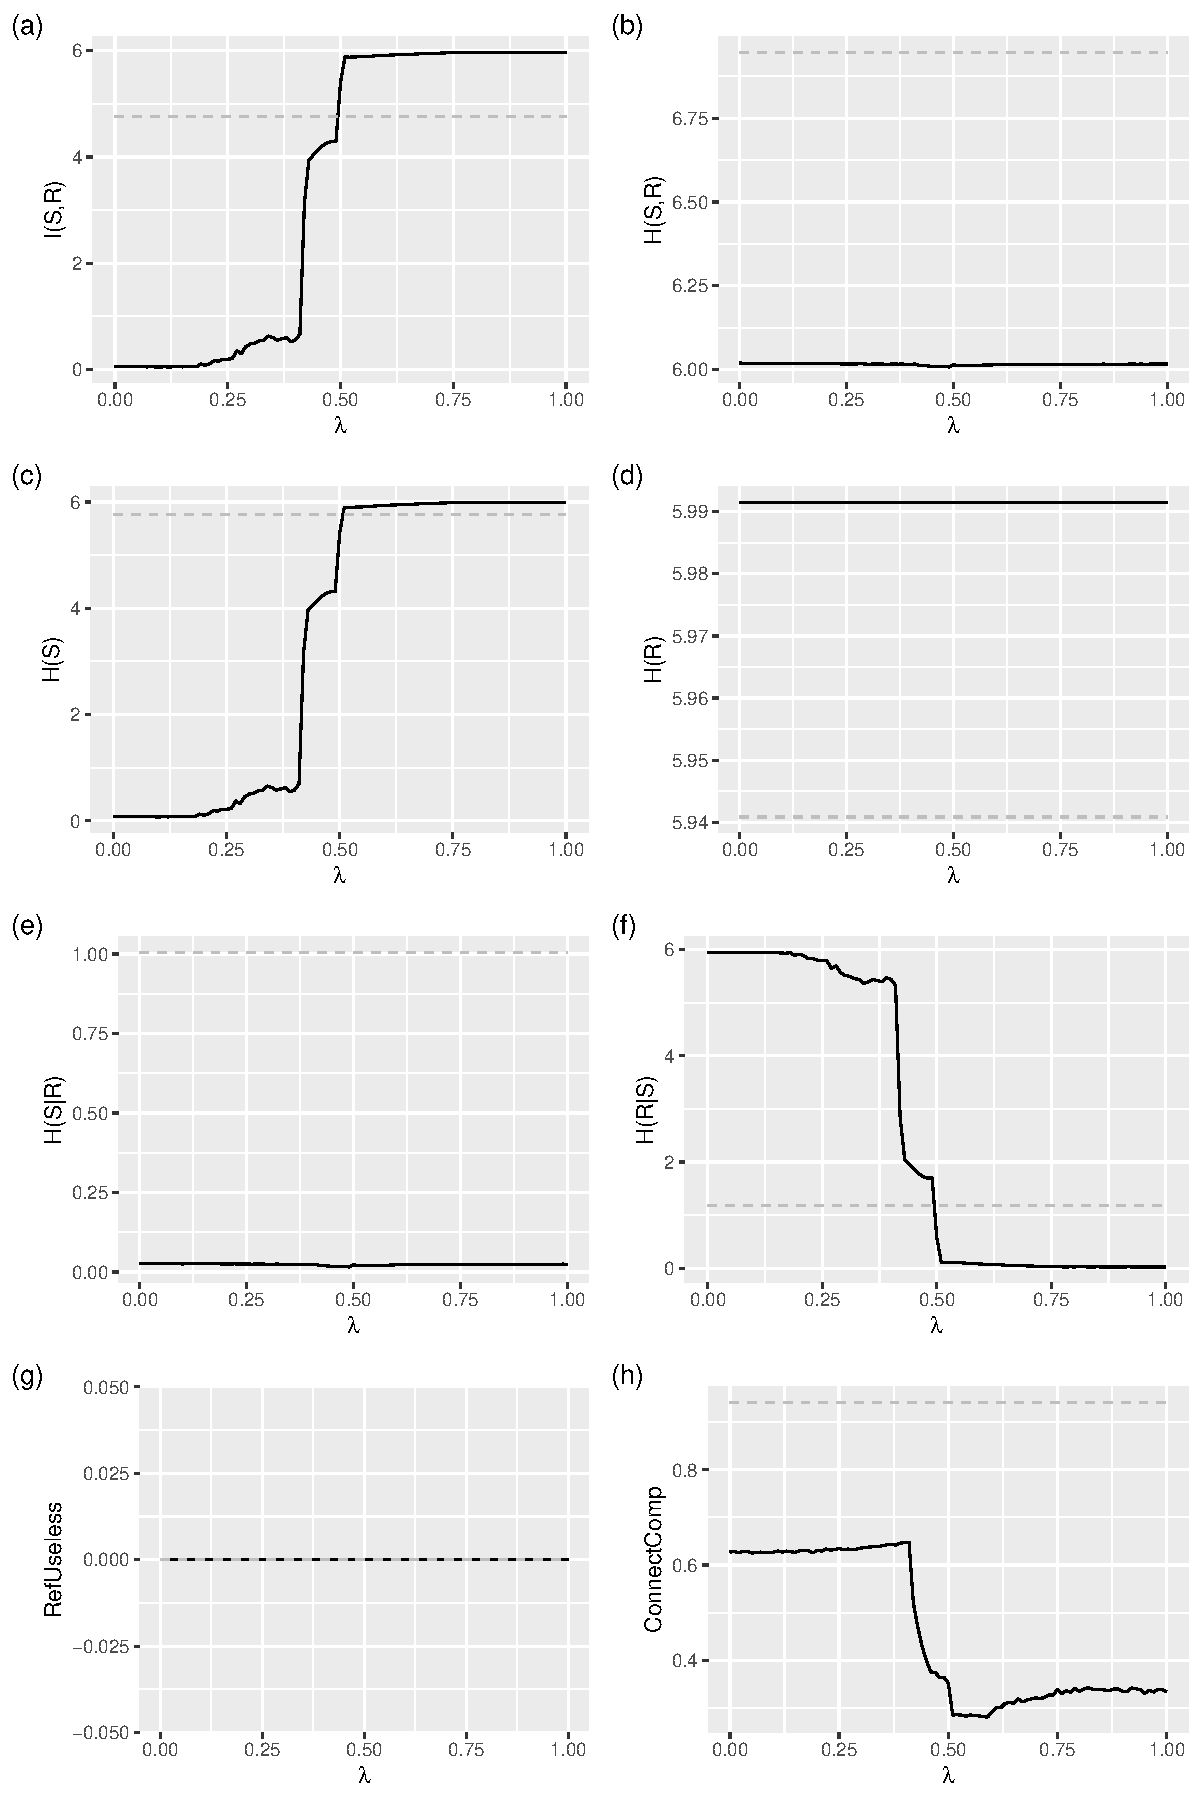
\includegraphics[width=\textwidth]{informationTheoretic_uniform_phi0_nm400_dynamic_randomBipartite_disallowUnlinked}
  \caption{Same information as in Figure \ref{fig:informationTheoretic_uniform_phi0_nm400_dynamic_randomBipartite_allowUnlinked} but disconnected meanings are disallowed.}
  \label{fig:informationTheoretic_uniform_phi0_nm400_dynamic_randomBipartite_disallowUnlinked}
\end{figure}

\begin{figure}
  \centering
  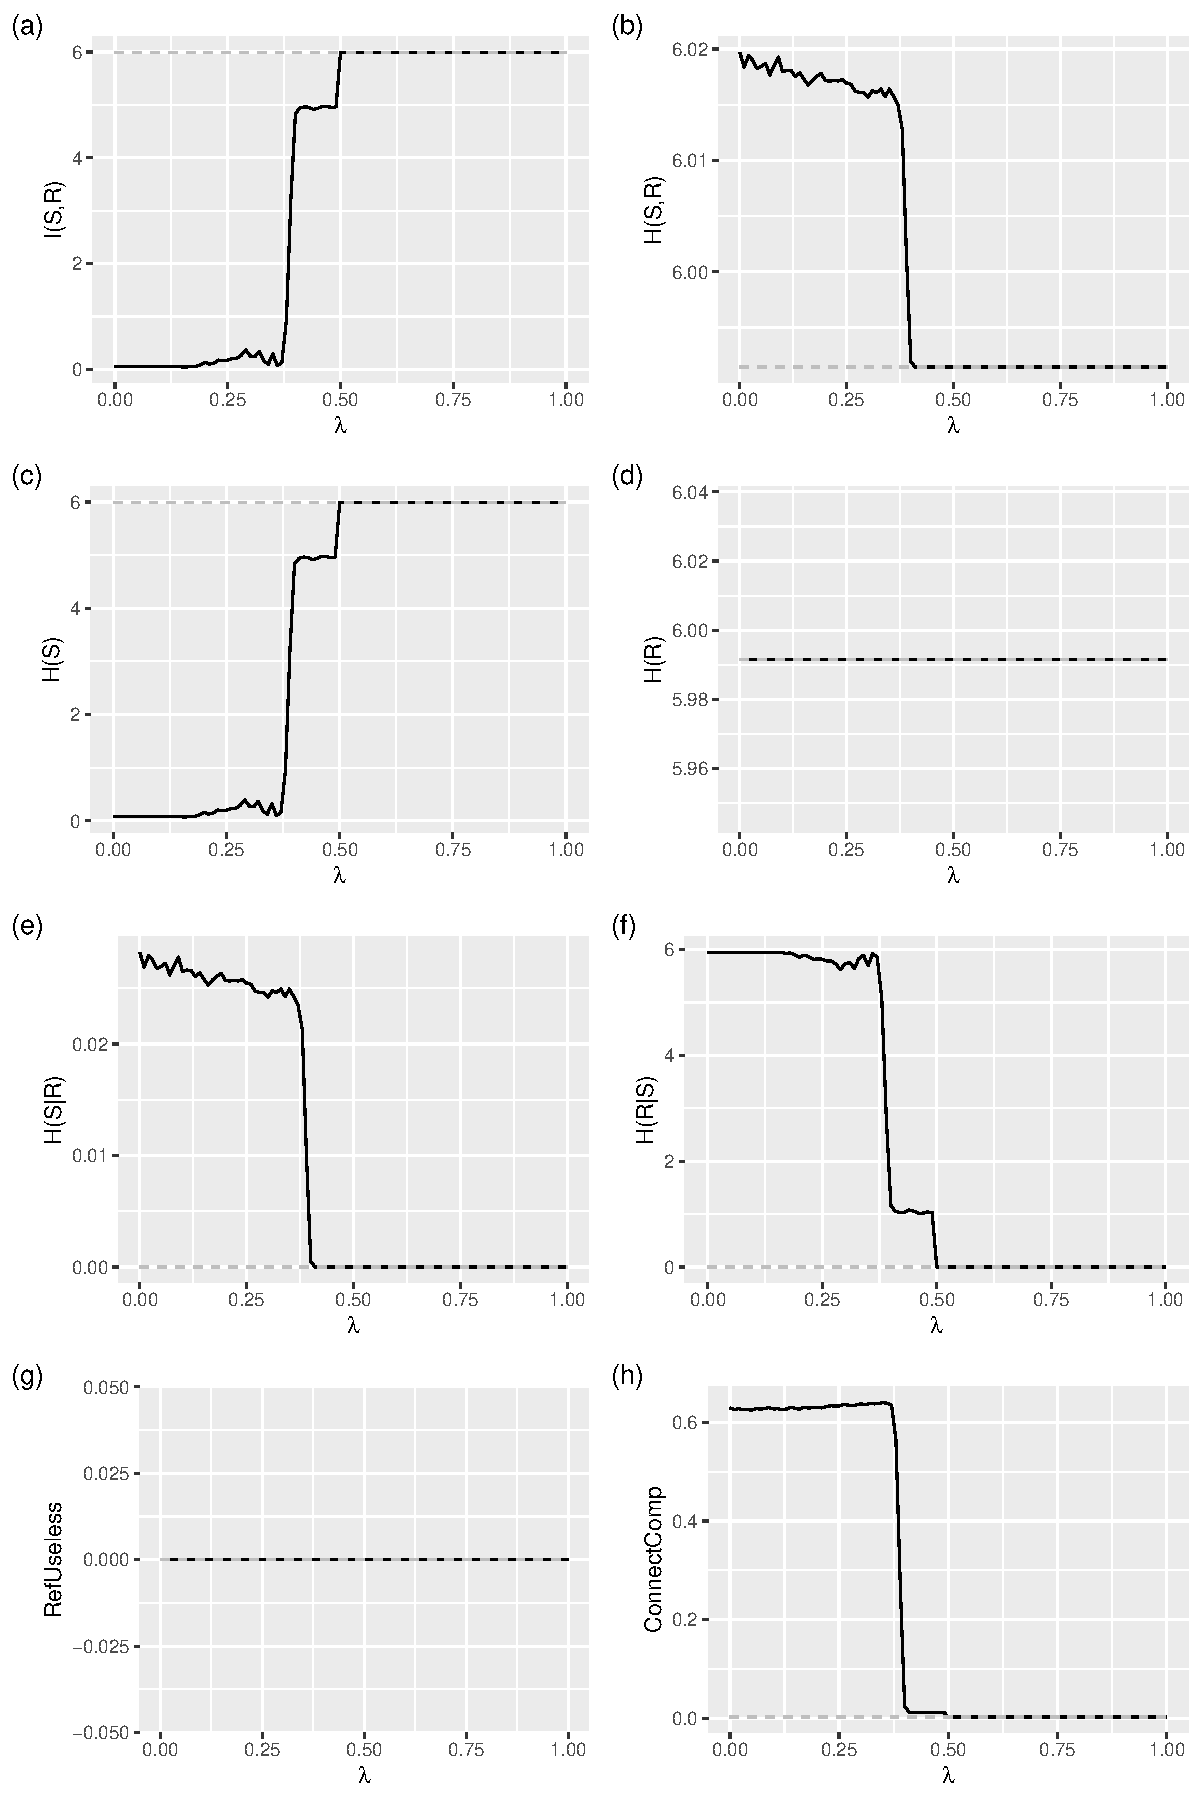
\includegraphics[width=\textwidth]{informationTheoretic_uniform_phi0_nm400_dynamic_oneToOne_disallowUnlinked}
  \caption{Same information as in Figure \ref{fig:informationTheoretic_uniform_phi0_nm400_dynamic_oneToOne_allowUnlinked} but disconnected meanings are disallowed.}
  \label{fig:informationTheoretic_uniform_phi0_nm400_dynamic_oneToOne_disallowUnlinked}
\end{figure}

Figures \ref{fig:insideLambda_uniform_phi0_nm400_dynamic_randomBipartite_disallowUnlinked} and \ref{fig:insideLambda_uniform_phi0_nm400_dynamic_oneToOne_disallowUnlinked} (random and one to one respectively) show statistical measures for select values of $\lambda$, with figures \ref{fig:fitting_insideLambda_uniform_phi0_nm400_dynamic_randomBipartite_disallowUnlinked} and \ref{fig:fitting_insideLambda_uniform_phi0_nm400_dynamic_oneToOne_disallowUnlinked} showing the fitting of the curve to a power law for a select value of $\lambda$.
None of the studied values of $\lambda$ between 0.49 and 0.5 resulted in a power law.
Tables \ref{tab:fitting_insideLambda_uniform_phi0_nm400_dynamic_randomBipartite_disallowUnlinked} and \ref{tab:fitting_insideLambda_uniform_phi0_nm400_dynamic_oneToOne_disallowUnlinked} show the values of the regression's exponent and factor

\begin{figure}
  \centering
  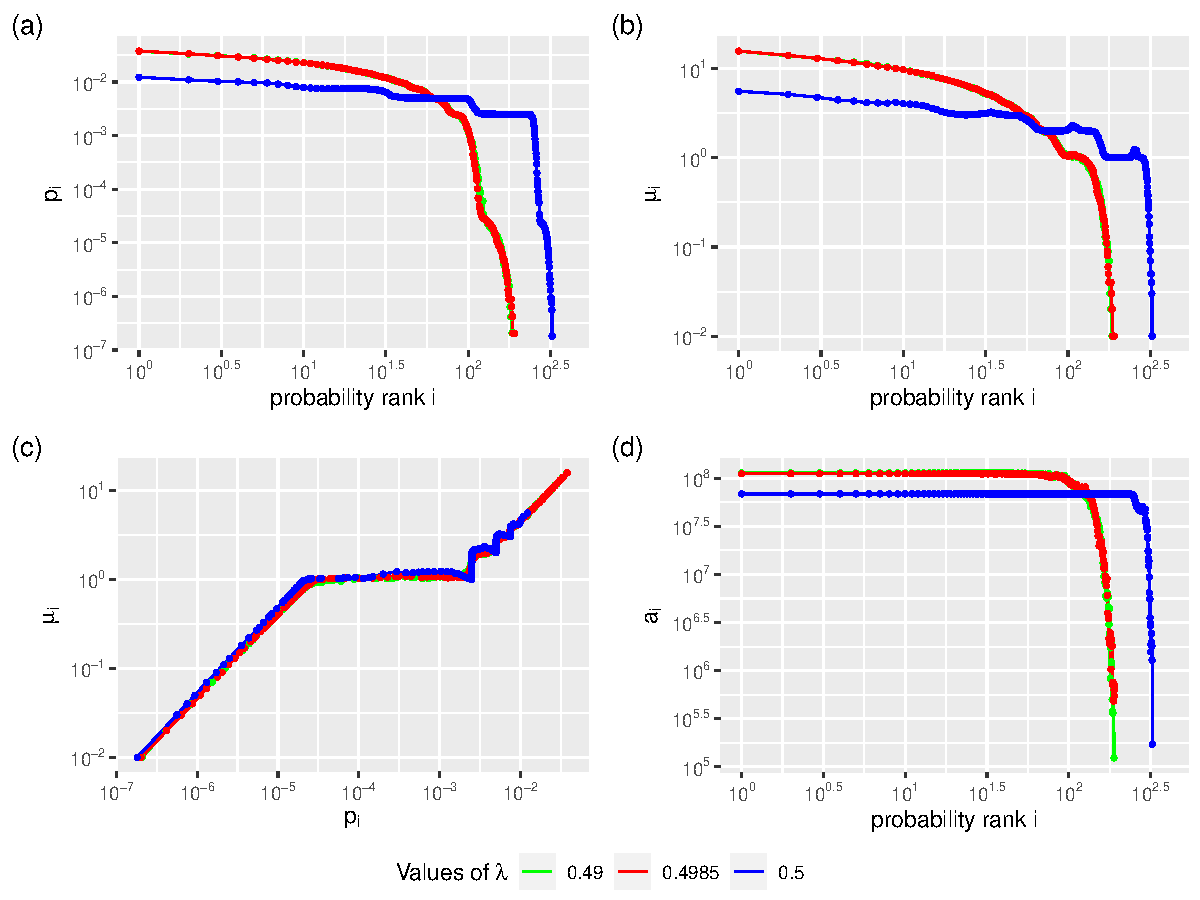
\includegraphics[width=\textwidth]{insideLambda_uniform_phi0_nm400_dynamic_randomBipartite_disallowUnlinked}
  \caption{Same information as in Figure \ref{fig:insideLambda_uniform_phi0_nm400_dynamic_randomBipartite_allowUnlinked} but disconnected meanings are disallowed.}
  \label{fig:insideLambda_uniform_phi0_nm400_dynamic_randomBipartite_disallowUnlinked}
\end{figure}

\begin{figure}
  \centering
  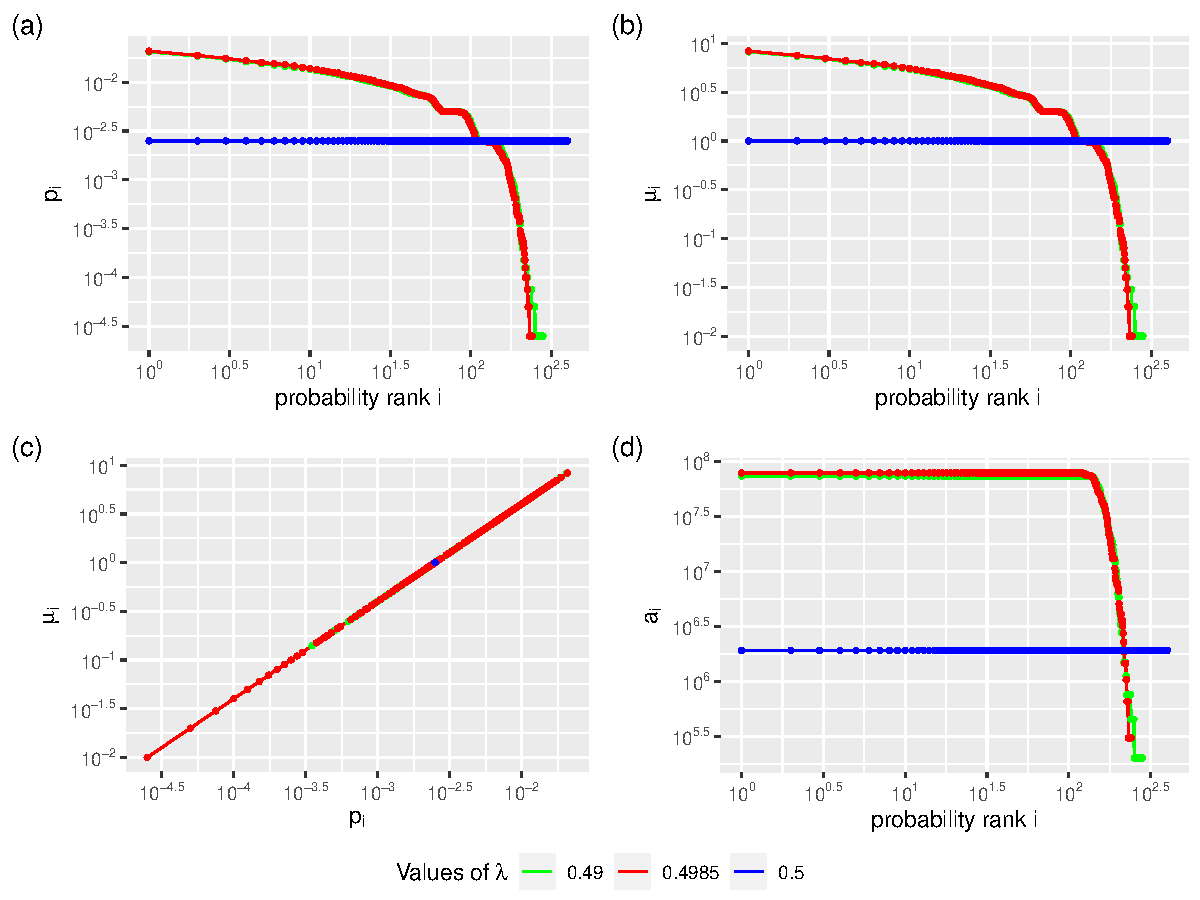
\includegraphics[width=\textwidth]{insideLambda_uniform_phi0_nm400_dynamic_oneToOne_disallowUnlinked}
  \caption{Same information as in Figure \ref{fig:insideLambda_uniform_phi0_nm400_dynamic_oneToOne_allowUnlinked} but disconnected meanings are disallowed.}
  \label{fig:insideLambda_uniform_phi0_nm400_dynamic_oneToOne_disallowUnlinked}
\end{figure}

\begin{figure}
  \centering
  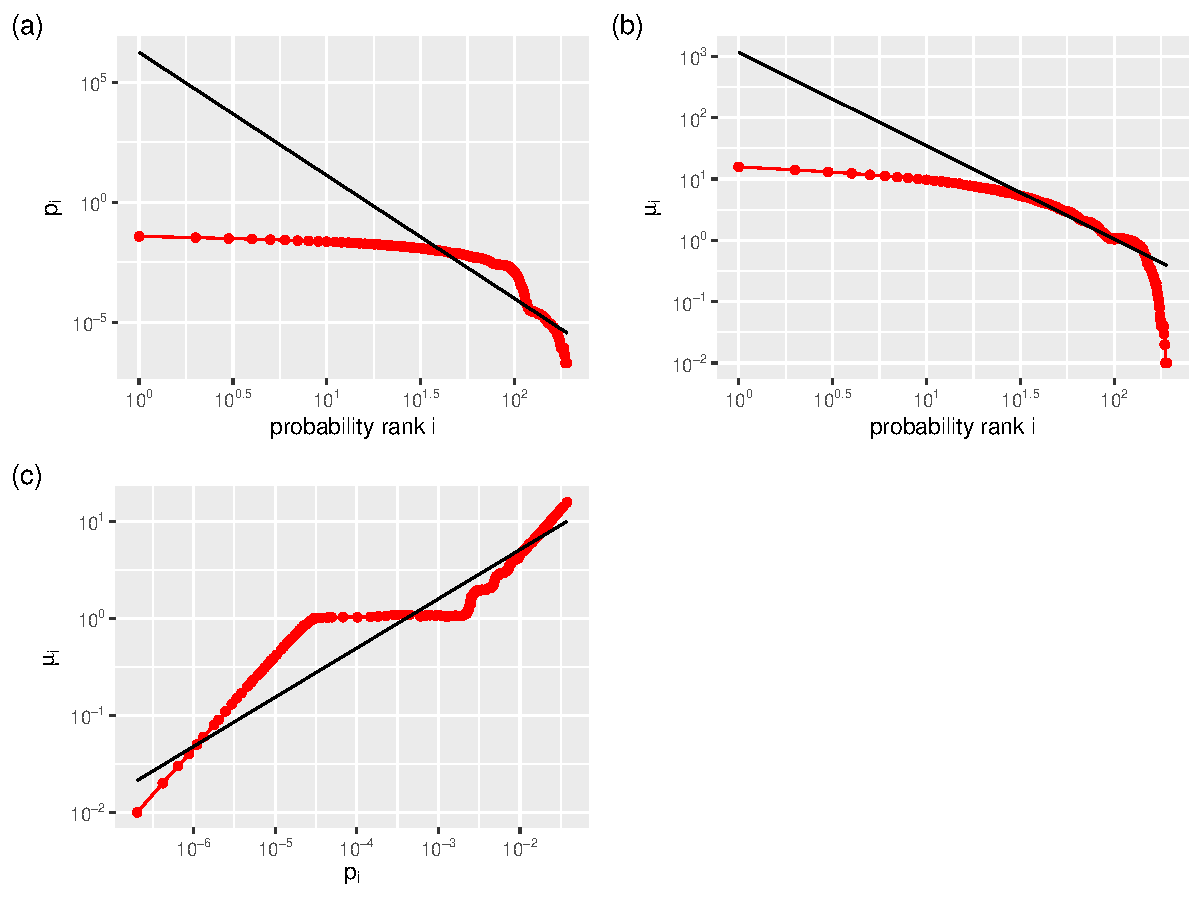
\includegraphics[width=\textwidth]{fitting_insideLambda_uniform_phi0_nm400_dynamic_randomBipartite_disallowUnlinked}
  \caption{Same information as in Figure \ref{fig:fitting_insideLambda_uniform_phi0_nm400_dynamic_randomBipartite_allowUnlinked} but disconnected meanings are disallowed.
Table \ref{tab:fitting_insideLambda_uniform_phi0_nm400_dynamic_randomBipartite_disallowUnlinked} shows the values of the exponent and the factor of the fitted power law.}
  \label{fig:fitting_insideLambda_uniform_phi0_nm400_dynamic_randomBipartite_disallowUnlinked}
\end{figure}

\begin{figure}
  \centering
  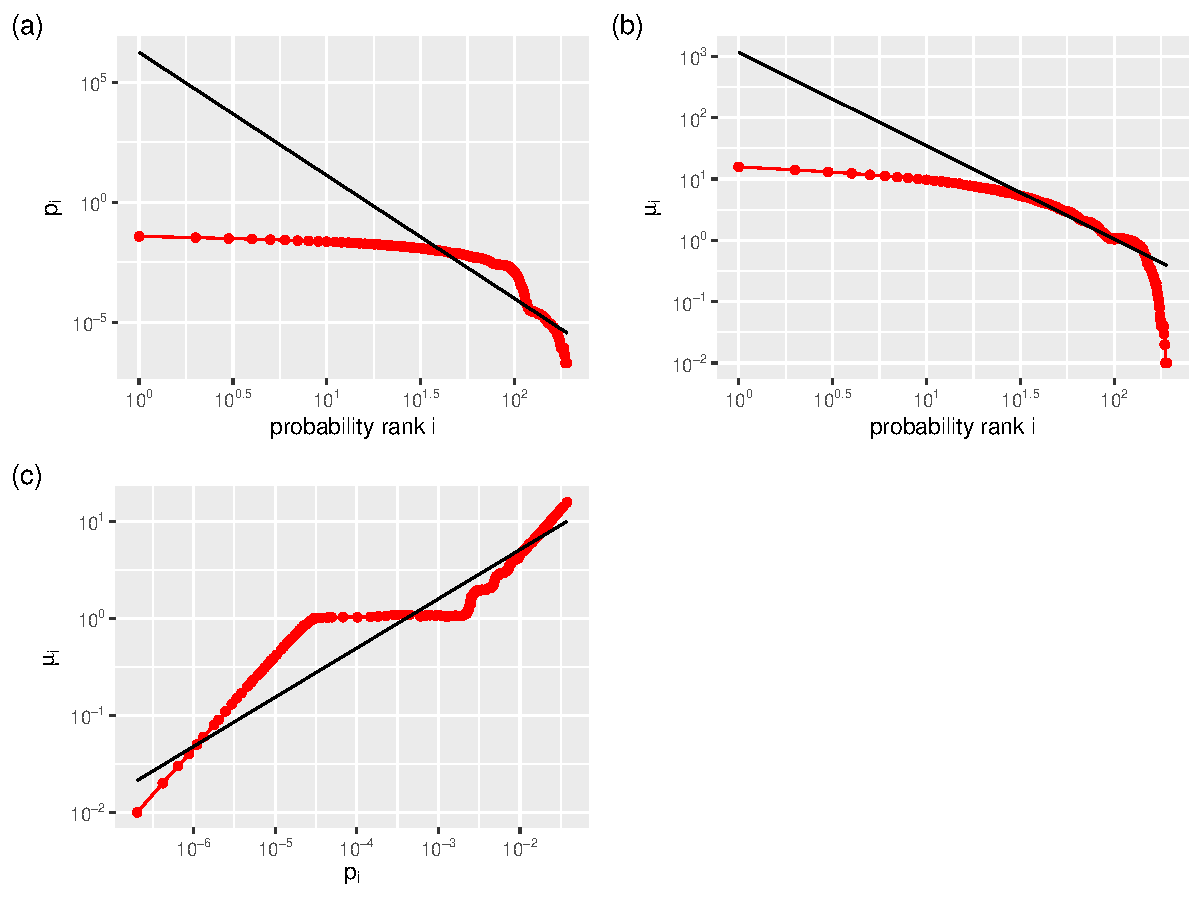
\includegraphics[width=\textwidth]{fitting_insideLambda_uniform_phi0_nm400_dynamic_oneToOne_disallowUnlinked}
  \caption{Same information as in Figure \ref{fig:fitting_insideLambda_uniform_phi0_nm400_dynamic_oneToOne_allowUnlinked} but disconnected meanings are disallowed.
Table \ref{tab:fitting_insideLambda_uniform_phi0_nm400_dynamic_oneToOne_disallowUnlinked} shows the values of the exponent and the factor of the fitted power law.}
  \label{fig:fitting_insideLambda_uniform_phi0_nm400_dynamic_oneToOne_disallowUnlinked}
\end{figure}

% latex table generated in R 4.1.1 by xtable 1.8-4 package
% Tue Oct  5 00:38:21 2021
\begin{table}[ht]
\centering
\begin{tabular}{lrr}
  \hline
plot & $\alpha$ & $k$ \\ 
  \hline
a & 5.1239660 & 1744404.5869742 \\ 
  b & 0.1949778 & 0.0413557 \\ 
  c & 1.5237337 & 1164.4863367 \\ 
  d & -0.5072076 & 52.8958272 \\ 
  f & 1.5439705 & 1287.7147444 \\ 
  g & 0.8441915 & 0.2950000 \\ 
   \hline
\end{tabular}
\caption{Table showing the exponent and factor of the power laws fitted in Figure \ref{fig:fitting_insideLambda_uniform_phi0_nm400_dynamic_randomBipartite_disallowUnlinked}} 
\label{tab:fitting_insideLambda_uniform_phi0_nm400_dynamic_randomBipartite_disallowUnlinked}
\end{table}


\begin{table}
  \centering
  \begin{adjustbox}{max width=\textwidth}
    \begin{tabular}{llSS}
      \toprule
      plot & law & $a$ & $k$ \\ 
      \midrule
      a & word frequency & 1.6856845 & 5.9091866 \\ 
      b & \redtxt{word frequency (cumulative)} & 0.5677904 & 0.0082092 \\ 
      c & meaning distribution & 1.6856845 & 2363.6746229 \\ 
      d & meaning frequency & -1.0000000 & 400.0000000 \\ 
      f & \redtxt{meaning distribution} & 1.6856845 & 2363.6746229 \\ 
      g & \redtxt{meaning distribution (cumulative)} & 1.3451676 & 0.4195512 \\ 
      \bottomrule
    \end{tabular}
  \end{adjustbox}    
  \caption{\redtxt{en vermell: cal mostrar?} Table showing the exponent and factor of the power laws fitted in Figure \ref{fig:fitting_insideLambda_uniform_phi0_nm400_dynamic_oneToOne_disallowUnlinked}} 
  \label{tab:fitting_insideLambda_uniform_phi0_nm400_dynamic_oneToOne_disallowUnlinked}
\end{table}

%%% Local Variables:
%%% mode: latex
%%% TeX-master: "../tfm"
%%% End:


For the case $\phi=1$, Figures \ref{fig:informationTheoretic_uniform_phi1_nm400_dynamic_randomBipartite_disallowUnlinked} and \ref{fig:informationTheoretic_uniform_phi1_nm400_dynamic_oneToOne_disallowUnlinked} show the information theoretical measures of the optimal graph for values of $\lambda$ ranging from 0 to 1. They correspond to the initial graph being a random bipartite graph and a one to one configuration respectively. It is interesting to see that when $\phi=1$ the one to one configuration fails to evolve for any value of $\lambda$.

\begin{figure}
  \centering
  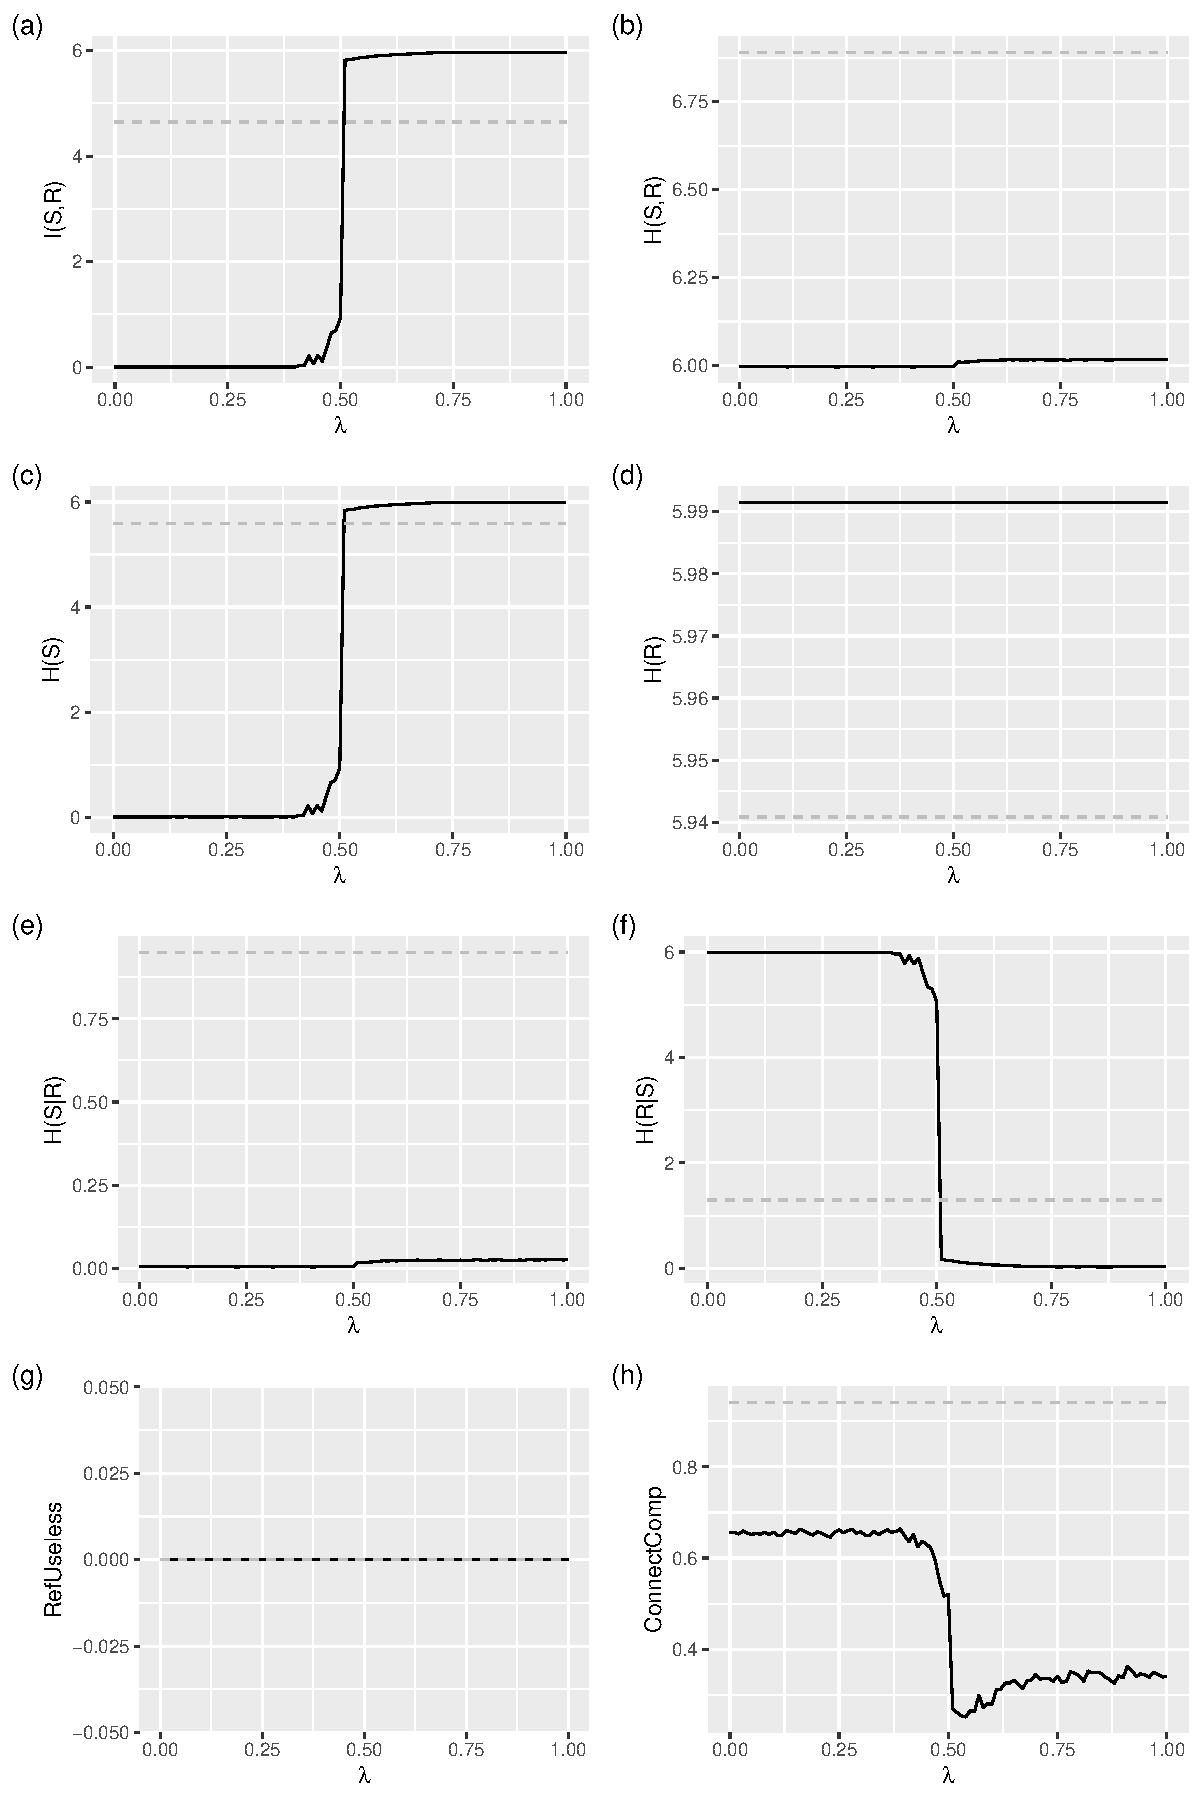
\includegraphics[width=\textwidth]{informationTheoretic_uniform_phi1_nm400_dynamic_randomBipartite_disallowUnlinked}
  \caption{Same information as in Figure \ref{fig:informationTheoretic_uniform_phi1_nm400_dynamic_randomBipartite_allowUnlinked} but disconnected meanings are disallowed.}
  \label{fig:informationTheoretic_uniform_phi1_nm400_dynamic_randomBipartite_disallowUnlinked}
\end{figure}

\begin{figure}
  \centering
  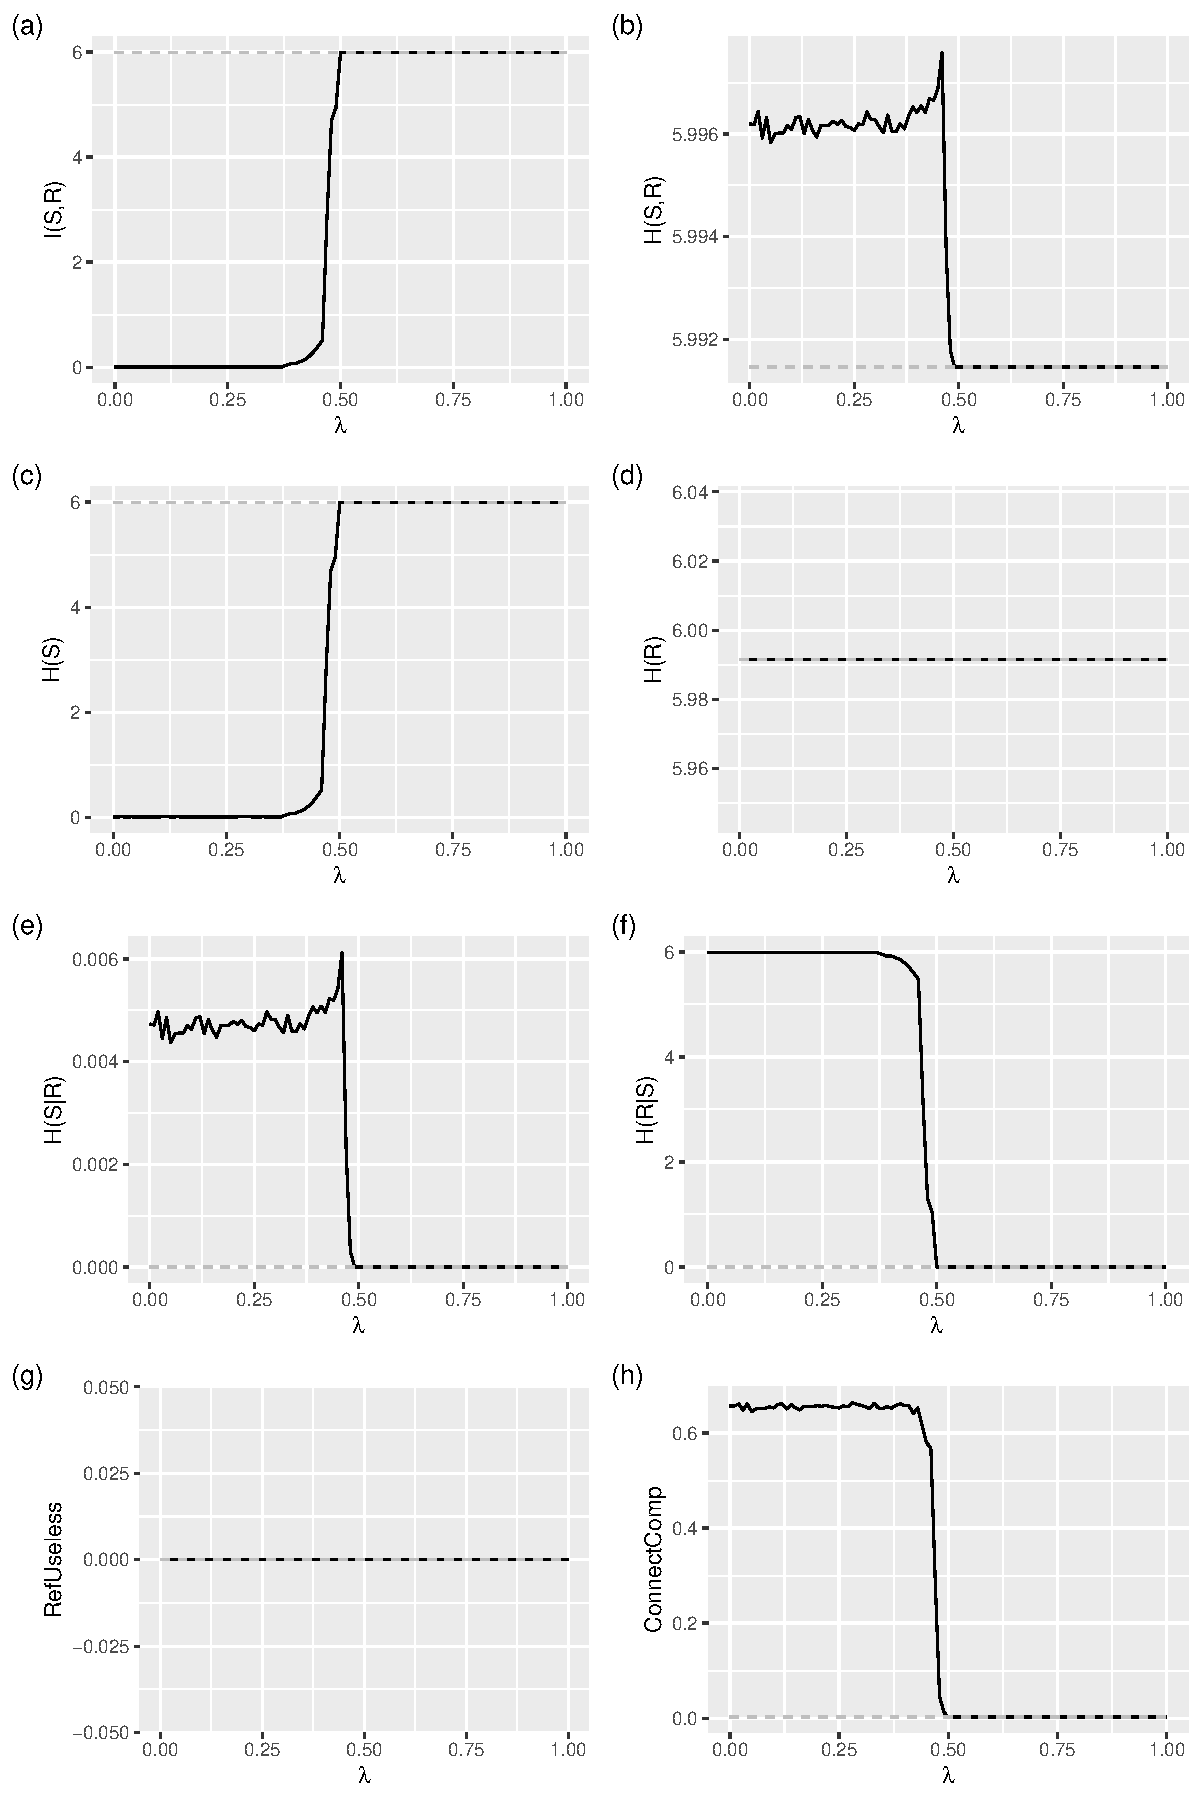
\includegraphics[width=\textwidth]{informationTheoretic_uniform_phi1_nm400_dynamic_oneToOne_disallowUnlinked}
  \caption{Same information as in Figure \ref{fig:informationTheoretic_uniform_phi1_nm400_dynamic_oneToOne_allowUnlinked} but disconnected meanings are disallowed.}
  \label{fig:informationTheoretic_uniform_phi1_nm400_dynamic_oneToOne_disallowUnlinked}
\end{figure}

Figure \ref{fig:insideLambda_uniform_phi0_nm400_dynamic_randomBipartite_disallowUnlinked} shows statistical measures for select values of $\lambda$, with figure \ref{fig:fitting_insideLambda_uniform_phi0_nm400_dynamic_randomBipartite_disallowUnlinked} showing the fitting of the curve to a power law for a select value of $\lambda$.
Table \ref{tab:fitting_insideLambda_uniform_phi0_nm400_dynamic_randomBipartite_disallowUnlinked} shows the values of the regression's exponent and factor

\begin{figure}
  \centering
  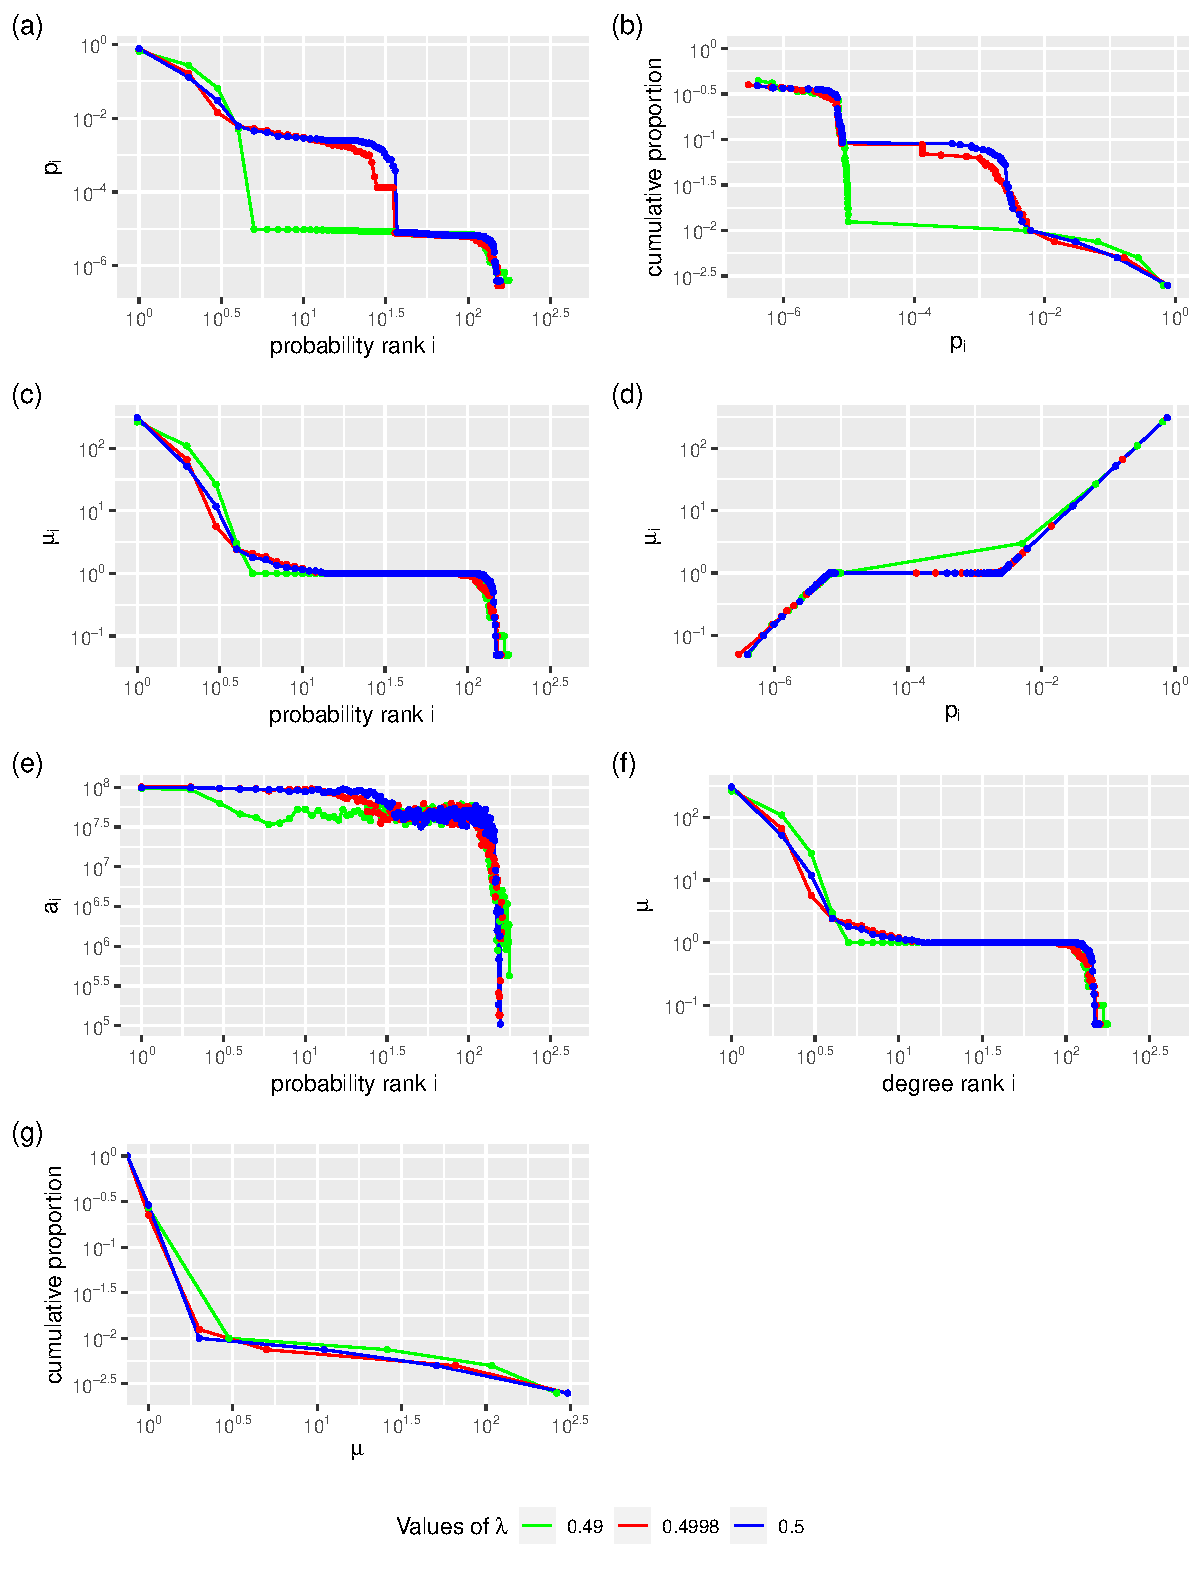
\includegraphics[width=\textwidth]{insideLambda_uniform_phi1_nm400_dynamic_randomBipartite_disallowUnlinked}
  \caption{Same information as in Figure \ref{fig:insideLambda_uniform_phi1_nm400_dynamic_randomBipartite_allowUnlinked} but disconnected meanings are disallowed.}
  \label{fig:insideLambda_uniform_phi1_nm400_dynamic_randomBipartite_disallowUnlinked}
\end{figure}

\begin{figure}
  \centering
  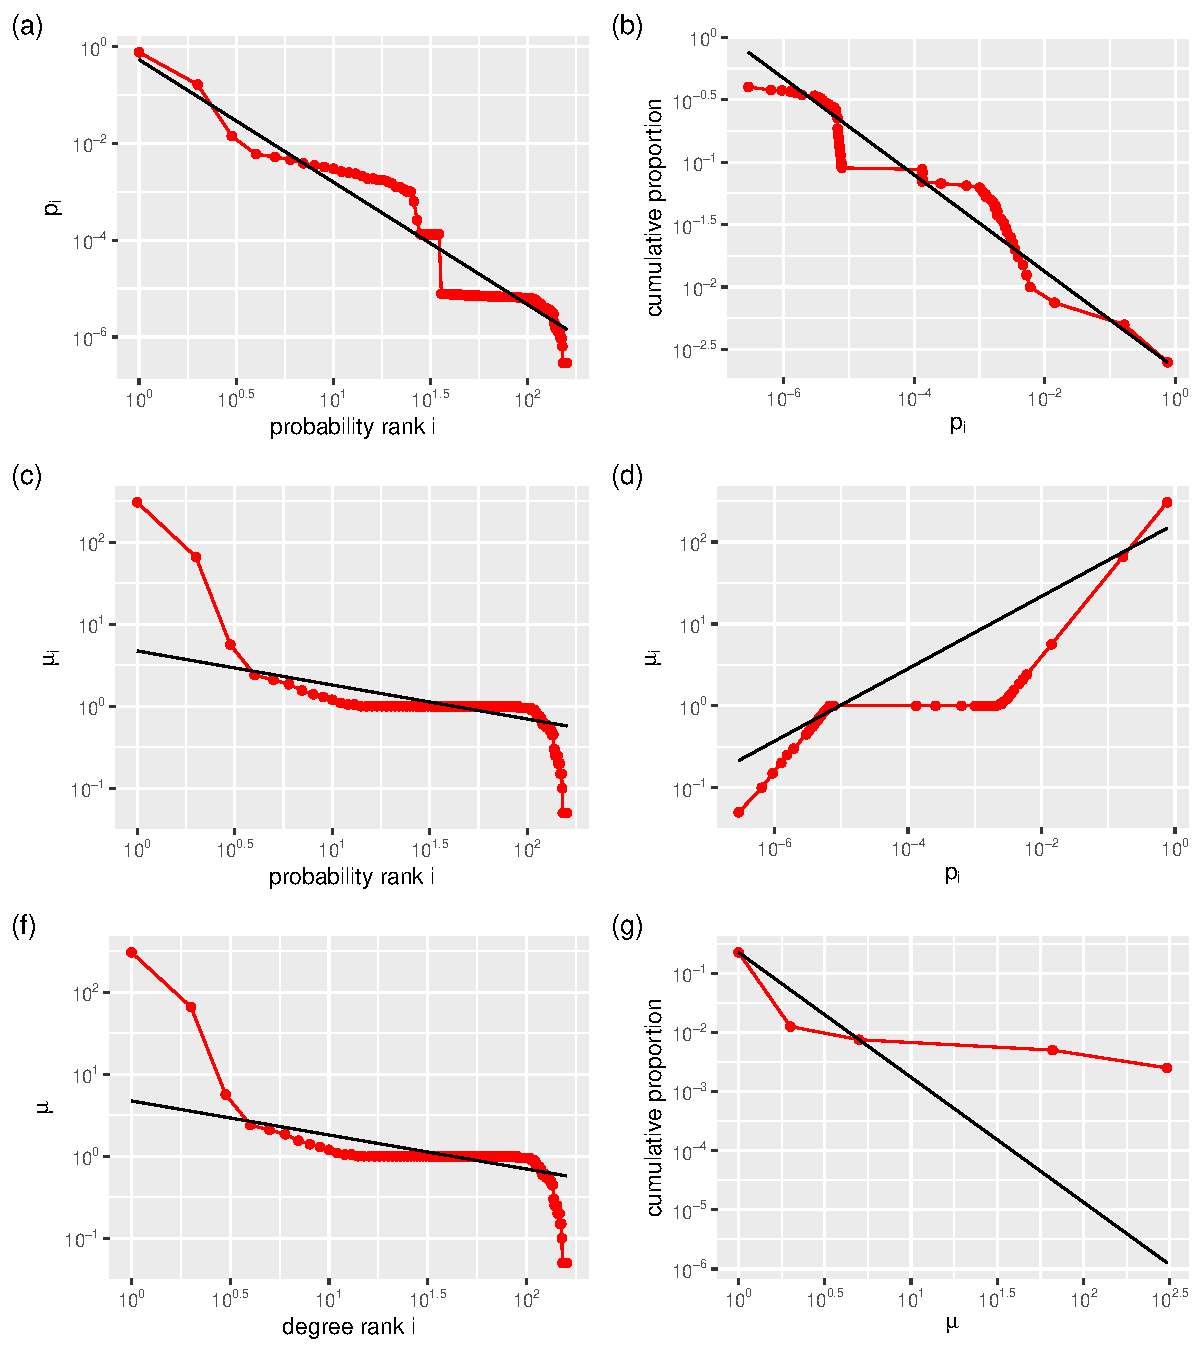
\includegraphics[width=\textwidth]{fitting_insideLambda_uniform_phi1_nm400_dynamic_randomBipartite_disallowUnlinked}
  \caption{Same information as in Figure \ref{fig:fitting_insideLambda_uniform_phi1_nm400_dynamic_randomBipartite_allowUnlinked} but disconnected meanings are disallowed.
Table \ref{tab:fitting_insideLambda_uniform_phi1_nm400_dynamic_randomBipartite_disallowUnlinked} shows the values of the exponent and the factor of the fitted power law.}
  \label{fig:fitting_insideLambda_uniform_phi1_nm400_dynamic_randomBipartite_disallowUnlinked}
\end{figure}

\begin{table}
  \centering
  \begin{adjustbox}{max width=\textwidth}
    \begin{tabular}{llSS[scientific-notation=true]}
      \toprule
      plot & law & $a$ & $k$ \\ 
      \midrule
      a & word frequency ($\alpha$) & 2.5318774 & 0.5389468 \\ 
      %b & \redtxt{word frequency (cumulative)} & 0.3865160 & 0.0022479 \\ 
      b & meaning distribution ($\gamma$) & 0.4151170 & 4.7225143 \\ 
      c & meaning frequency ($\delta$) & -0.4419160 & 166.3791217 \\ 
      %f & \redtxt{meaning distribution} & 0.4151170 & 4.7225143 \\ 
      %g & \redtxt{meaning distribution (cumulative)} & 2.1132828 & 0.2250000 \\ 
      \bottomrule
    \end{tabular}
  \end{adjustbox}
  \caption{Table showing the exponent and factor of the power laws fitted for the \secondmodel{} with $\phi=1$, disallowed unlinked meanings and a random bipartite graph as the initial condition (Figure \ref{fig:fitting_insideLambda_uniform_phi1_nm400_dynamic_randomBipartite_disallowUnlinked})
    In this table, $\alpha \approx 2.5$, $\delta \approx 0.44$ and $\gamma \approx 0.4$.
    The relationship between these values (Equation \eqref{eq:relation-exponents}) does not hold.
    The exponent for $\alpha$ are not exactly the one expected, however both $\gamma$ and $\delta$ are very close to the expected $1/2$.
  } 
  \label{tab:fitting_insideLambda_uniform_phi1_nm400_dynamic_randomBipartite_disallowUnlinked}
\end{table}

%%% Local Variables:
%%% mode: latex
%%% TeX-master: "../tfm"
%%% End:


%%% Local Variables:
%%% mode: latex
%%% TeX-master: "tfm"
%%% End:
